\documentclass[letterpaper, 12 pt, conference]{ieeeconf}

\usepackage{siunitx}
\usepackage{graphicx}
\usepackage[utf8]{inputenc}
\usepackage[T1]{fontenc}
\usepackage{subfigure, siunitx, url}
\usepackage{amsmath, amssymb, bbm, nicefrac}
\usepackage{pifont}
%\usepackage{tikz}
%\usetikzlibrary{shapes,arrows,fit,trees,positioning,chains,calc,intersections}

%%% abbreviations to use (guarantee correct spaces between characters)
\newcommand{\ie}{i.e.\ }
\newcommand{\Ie}{I.e.\ }
\newcommand{\eg}{e.g.\ }
\newcommand{\Eg}{E.g.\ }
\newcommand{\cf}{cf.}

%%% commands for referencing (guarantee homogeneous writing style)
\newcommand{\referenceChapter}[1]{Chapter \ref{#1}}
\newcommand{\referenceSection}[1]{Section \ref{#1}}
\newcommand{\referenceFigure}[1]{Figure \ref{#1}}
\newcommand{\referenceEquation}[1]{Eq.~(\ref{#1})}
\newcommand{\referenceTable}[1]{Table \ref{#1}}
\newcommand{\referenceListing}[1]{code listing\ref{#1}}
\newcommand{\referenceAlgorithm}[1]{Algorithm \ref{#1}}

\title{\LARGE \bf
CSCI 4155 Machine Learning\\\small “To Follow The Wall Or Not To Follow The Wall”…ask all the questions you want the robot will do what it wants…\\*
}


\author{Alexander Moriarty, Warren Okanski\\~\\~
        Intro to Machine Learning: Assignment 2\\
        Dalhousie University\\ 
        Halifax, Nova Scotia, Canada\\
        {\tt\small \{alexander, <unknown>\}@dal.ca}
}

\begin{document}

\maketitle

\begin{abstract}
The purpose of this lab was to investigate the use of the Proportional Integral Derivative controller algorithm in a wall-following robot exercise. A Proportional Integral Derivative controller, also known as a PID controller, utilizes the variance between the desired state of the function and the actual state of the function (the robot's behaviour being the function in this case) and is represented by \referenceEquation{pid-function}.
\end{abstract}


% \footnote{lkjasdlkj}

%\begin{figure}[tbp]
%\centering
%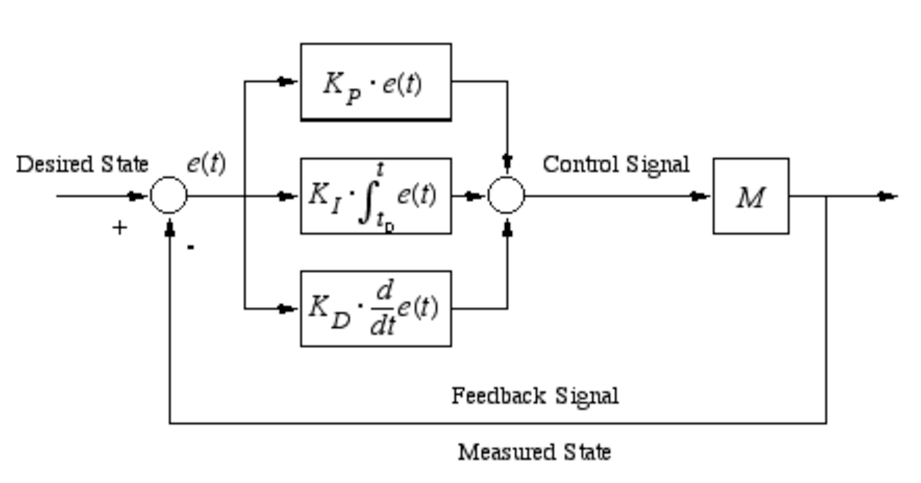
\includegraphics[width=0.5\textwidth]{images/pid.pdf}
%\caption{\label{pid-controller} PID controller}
%\end{figure}

\begin{equation}\label{pid-function}
u(t) = K_{P} e(t) + K_{I} \int_0^t e(t)\,dt + K_{D} \frac{d e(t)}{dt}
\end{equation}

\section{Introduction}\label{section_one}
Each of the three aspects of the controller represents a separate property of the error being computed. The proportional component represents the current error of the system. It is multiplied by a proportional constant and produces a value that defines the amount of response to a change in the system. Increasing the proportional component’s representation by increasing the proportional constant will create more of a response to some deviation from the desired state, however setting this constant too high can cause the system to become unstable in its attempts to adapt and too low can result in a high error to output ratio, creating insufficient attempts to reach the desired state. The integral component calculates the sum of the error of the system as time progresses. Similar to the proportional term, it is affected by an integral constant that may be adjusted to increase or decrease its contribution to the overall function. The integral component is especially useful for the PID controller as its output value relies on the previous error of the system and (in theory) maintains a decreasing but constant error that is required to drive the process, however, this creates an infinite overshooting of the desired state from the actual state of the function. Finally, the derivative component measures the slope of the change in error over time and uses this value to predict the response needed to correct the error. It is multiplied by a derivative constant that defines the magnitude of contribution by the derivative component to the overall function. In essence the derivative component determines the rate of adjustment to the error in the system and is effective at reducing the overshooting issue caused by the integral component. Unfortunately the derivative component amplifies noise in the error which can be problematic if the derivative constant is large. 



\section{Implementation}\label{section_implementation}
Implementation of the PID controller function was straight forward. The time consuming part of the process was finding optimal values for the constants $K_{P}$, $K_{I}$ and $K_{D}$ seen in \referenceEquation{pid-function}. During this process, we also tried different methods to avoid erroneous values. After testing with sampling and averaging, we decided not to because very little difference was noticed. Instead we returned to only adjusting the constants $K_{P}$, $K_{I}$ and $K_{D}$. Where our robot fails frequently is when the distance from the robot to the instantaneous center of rotation is less than the distance from the robot to the wall. In this case, once the robot start to turn towards the wall, the sonar value increases even though the robot is actually closer to the wall. Resulting in the robot turning faster towards the wall. We discussed methods which we could fix this, a second ultrasonic sensor would be ideal. In the end we found values for the constants that worked to our satisfaction most of the time. 

\section{Observations}\label{section_two}
\begin{figure}[tbd]
\centering
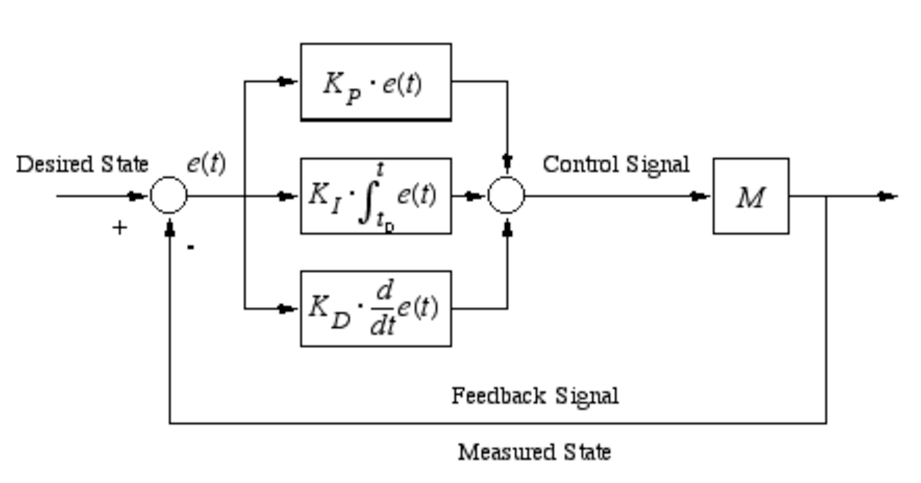
\includegraphics[width=0.5\textwidth]{images/pid.pdf}
\caption{\label{pid-controller} PID controller}
\end{figure}

\referenceFigure{pid-controller} represents a PID controller system\footnote{Image Source: \url{http://www.floatingvectors.com}}. As is shown by the diagram the difference between the ‘desired state’ and the ‘actual state’ (‘measured state’) is determined and calculated as the error of the system. This value is then processed by the PID controller and an output signal is sent to the device (often referred to as the Plant). The Plant then responds to the signal and using any sensors it is equipped with, produces a feedback signal dictating its new actual state. This cycle is looped until the desired state and the actual state functions are equivalent.

\section{Conclusion}\label{section_conclusion}
An interesting familiarity with this process occurs in neurological studies of sensory and motor processing in the human central nervous system.

\begin{figure}[!ht]
\centering
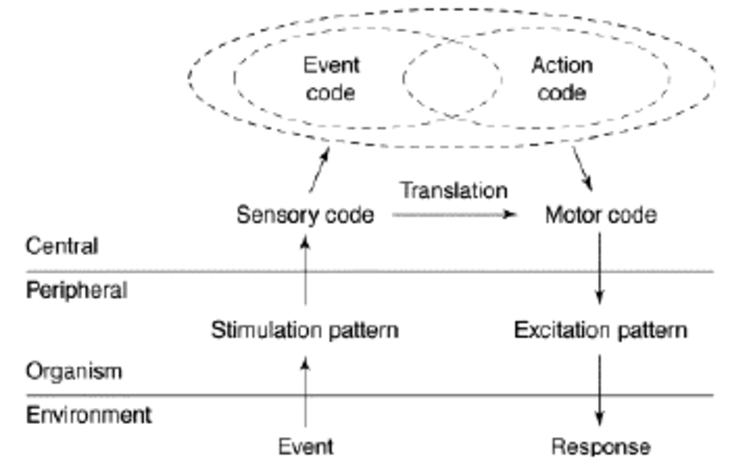
\includegraphics[width=0.5\textwidth]{images/neural-fig.pdf}
\caption{\label{neural-figure} Underlying neural mechanisms of sensory input to motor response.}
\end{figure}

\referenceFigure{neural-figure} demonstrates basic neural processes\footnote{Image Source: \url{http://www.sciencedirect.com}}
 associated with a change in the environment that are detected by human somatosensory signals to the brain, which are encoded and translated into motor signals that activate a motor response. The response is undoubtedly followed by a new change in environment and thus the cycle experienced with the PID controller system, is also observed in human everyday activity. This is one example of why it is so beneficial to acknowledge the similarities between both fields of study, where discoveries and advancements in one field may compliment or help advancements in the other. There is no doubt an obvious connection between human learning and machine learning, as machine learning is based on what we know of human neural processing, but identifying these connections is a helpful tool to understanding why things work the way they do or more importantly, why things aren't working the way they're expected to.


%%% REFERENCES %%%
\bibliography{literature_references}
\bibliographystyle{splncs}
%\bibliographystyle{plain}

%%% APPENDIX %%%

\end{document}





